Veel van de handmatige cijfers zijn te kraken door gebruik te maken frequentie analyse\index{Frequentie analyse}. Frequentie analyse is een techniek waarbij er gekeken wordt welke letters er in een taal in welke aantallen voorkomen. Door ervan uit te gaan dat elke encrypte tekst een gemiddelde verdeling heeft kunnen op basis van het voorkomen van bepaalde letters met een bepaalde frequentie de oorspronkelijke letters ingevuld worden. In figuur \ref{fig:NEfreq} staat de frequentie analyse van de Nederlandse taal. Hierbij is duidelijk dat de e de meest voorkomende letter is. Vinden we nu een encrypte tekst waarin p de meest voorkomende letter is dan kunnen we de p vervangen door de e. Als we zo alle letters af gaan dan kunnen we vele letters plaatsen en het bericht weer lezen.

\begin{figure}[h]
	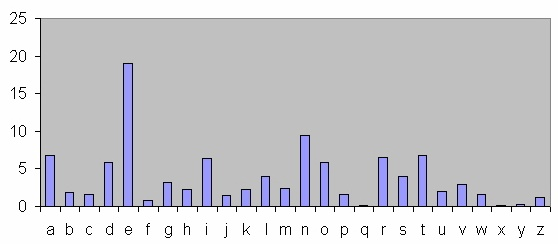
\includegraphics[width=\textwidth]{NEfreq.jpg}
	\caption{Frequentie Analyse van de Nederlandse taal (CC SA: Natastia at Dutch Wikipedia)}
	\label{fig:NEfreq}
\end{figure}

Met computers en digitale woordenboeken kunnen dit soort analyses heel snel gedaan worden. Het is natuurlijk wel belangrijk om te weten in wat voor taal het oorspronkelijke bericht was opgesteld.
